\chapter{自定义类型及其使用}
迄今为止,我们遇到的各种类型都是C++提供给我们的。要么是基本类型,要么是指针、数组、引用这样的复合类型。类型(Type)与数据(Data)之间是类与对象的关系。一个数据只不过是内存中若干 \lstinline@0@ 和 \lstinline@1@ 的排列组合,倘若没有类型,程序就不知道如何把这些信息解释成有效内容。而对于同一串 \lstinline@0@/\lstinline@1@ 来说,如果类型不同,那么解释出来的信息也是不一样的。以下是一个例子:
\begin{lstlisting}
    int n {0x63794b37}; //这是一个16进制字面量,其10进制为1668893495
    cout << (char*)&n; //以字符串形式输出
\end{lstlisting}
在某个环境下\footnote{不同环境下给出的结果不尽相同},它的输出是\\\noindent\rule{\linewidth}{.2pt}\texttt{
7KycT�\$��
}\\\noindent\rule{\linewidth}{.2pt}
为什么把 \lstinline@int*@ 类型转换成 \lstinline@char*@ 类型之后再输出就会得到这么奇怪的内容呢?原因就出在类型上。\par
\begin{figure}[htbp]
    \centering
    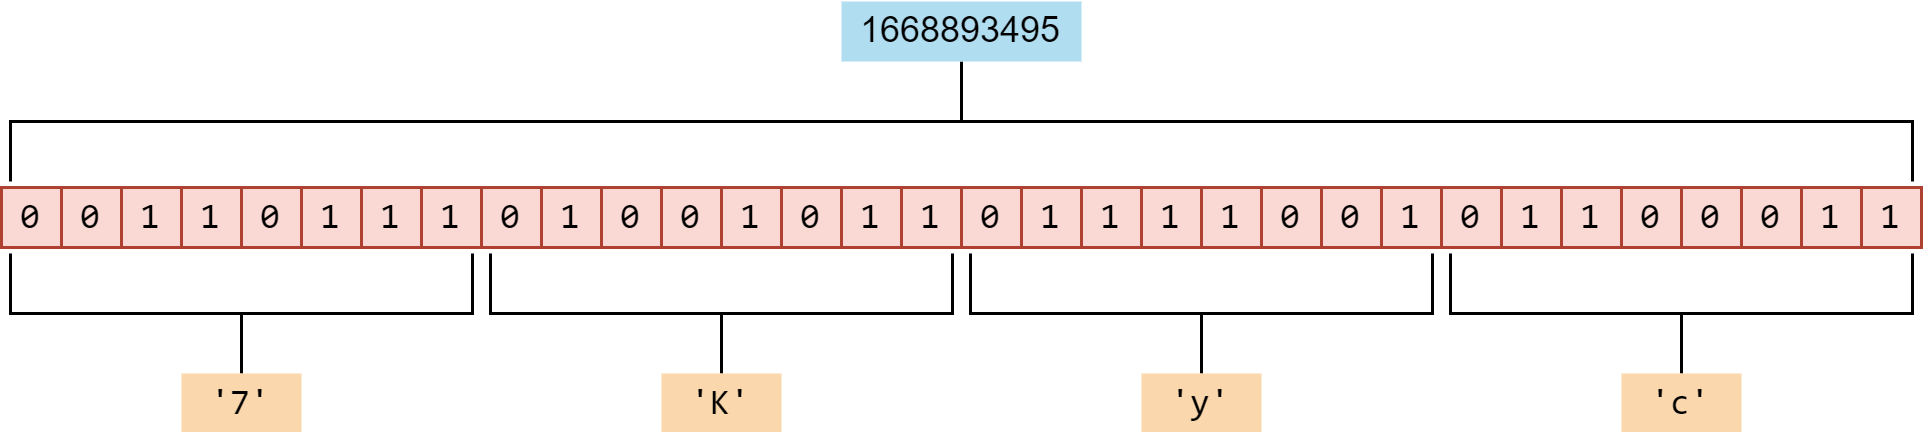
\includegraphics[width=\textwidth]{../images/generalized_parts/06_0_1_string_to_int_or_char.drawio.png}
    \caption{对同一段比特串,不同类型会解读出不同内容}
\end{figure}
内存中的32个比特如图所示。如果用 \lstinline@int@ 类型去解读它,就会得到 \lstinline@1668893495@;而如果用 \lstinline@char@ 类型去解读它,就会分别得到四个字符 \lstinline@'7'@, \lstinline@'K'@, \lstinline@'y'@, \lstinline@'c'@。而当我们以 \lstinline@char*@ 类型输出时,因为这里没有结束符 \lstinline@'\0'@,所以它还会继续输出后面内存中的无意义内容,直到碰到结束符为止。\par
所以我们可以认为,类型就是信息与二进制编码之间的一套转换方案。同样一串二进制编码,在不同类型下会解释出不同的信息——这也就是为什么我从第一章起就在强调``类型''。\par
那么言归正传(刚才的内容看不懂也没关系)。在本章,我将讲解如何利用基本数据类型和上一章中讲到的复合数据类型,来自创类型。我们不需要研究到比特这个层次,更不需要讲什么编码,我们拿C++现成的类型来组合就可以了。\par
\import{06_custom_types_and_their_use/}{01_enum.tex}
\import{06_custom_types_and_their_use/}{02_struct.tex}
\import{06_custom_types_and_their_use/}{03_exercise_example_list.tex}
\import{06_custom_types_and_their_use/}{04_union.tex}
\import{06_custom_types_and_their_use/}{05_introduction_to_class.tex}
